\section{Preliminary Evaluation}

In this section, we will first evaluate the effect of different types of
sequence predictor on the end-to-end parsing accuracy, and then compare
our parsing results with MSTParser and MaltParser on 8 different languages,
including ones with more non-projective features. We will also present the
parsing times of these different parsers.
%before finally outlining the demonstration of our system.


\subsection{Sequence Predictors}
We test the performance of parsing sequences generated by
different predictors along with two base lines: random sequence (Rand) and
left-to-right sequence from the sentence itself (L-to-R).
The end-to-end parsing accuracies are shown in \tabref{tab:seqtest}.
The training set is sections 2-21 of WSJ corpus and test set is sections 
00-01 of WSJ.  The final results show that Malt sequences provide 
the best performance. 
In fact, we observe that Malt sequences match the human intuition better,
which leads to a better overall result.
What's more, we explored an upper bound in accuracy of the proposed
sequence-based parsing framework, given our graph-based head mapper.
This upper bound of 93.59\% is achieved by using a gold sequence inferred from 
the gold parse of the test data (breadth-first traversal). 
\begin{table}[ht]
\small
  \centering
  \caption{Accuracies by different predictors}
    \begin{tabular}{lc}
    \toprule
    Sequence Predictor & Accuracy \\
    \midrule
    MaltSeq & \bf{89.50}\% \\
    PairwiseLTR & 77.84\% \\
    ScoreBased & 67.73\% \\
    Rand  & 70.92\% \\
    L-to-R & 63.36\% \\
    Gold Sequence (upper bound) & 93.59\% \\
    \bottomrule
    \end{tabular}%
  \label{tab:seqtest}%
\end{table}%
%\begin{table}[htbp]
%  \centering
%  \caption{Accuracy on different types of sequences}
%    \begin{tabular}{l|c|c|c|c}
%        \whline
%    \bf{Type} & Malt  & BF & Rand & L-to-R \\
%    \hline
%    \bf{Accu.} & {\bf 93.59\%} & 92.36\% & 70.92\% & 63.36\% \\
%    \whline
%    \end{tabular}%
%  \label{tab:seqtest}%
%\end{table}%

\subsection{Parsing accuracy}
% Table generated by Excel2LaTeX from sheet 'Sheet1'
We perform experiments on eight treebanks in different 
languages\footnote{\urlstyle{same}\url{http://ilk.uvt.nl/conll/post_task_data.html}}\footnote{\urlstyle{same}\url{http://www.nltk.org/nltk_data/}}.
The results shown in \tabref{tab:multilingual test} compare our best approach
(MaltSeq) with both Malt and MST.
%\BF{non-proj experiment}
\begin{table}[ht]
\small
    \centering
    \caption{End-to-end accuracies on 8 languages}
    \begin{tabular}{l|ccc}
        %\toprule
        \whline
        Language & MaltSeq & MST & Malt \\
        %\midrule
        \hline
        basque & 77.45\% & 81.81\% & 74.88\% \\
        catalan & 80.22\% & 82.18\% & 79.84\% \\
        danish & 86.84\% & 89.39\% & 85.65\% \\
        dutch & 81.43\% & 85.66\% & 77.28\% \\
        portuguese & 86.93\% & 88.63\% & 85.97\% \\
        slovene & 78.26\% & 80.16\% & 76.09\% \\
        swedish & 87.11\% & 88.12\% & 87.46\% \\
        english & 89.50\% & 90.64\% & 90.23\% \\
        %\bottomrule
        \whline
    \end{tabular}%
    \label{tab:multilingual test}%
\end{table}%
Generally, we outperform Malt in non-projective treebanks, 
which indicates that our framework tolerates free word order better. 
Graph-based method gives a better results for non-projective parsing 
than Malt, since it directly scores all arcs between every two nodes. 
Our accuracy is not as good as MST, because of the greedy decoding strategy.
Nevertheless, this strategy gives rise to improvement in 
parsing time and flexibility in defining high order features than MST.
This is only a preliminary result of our framework, more optimizations 
are expected in the further work.

\subsection{Parsing Time}

We measure the average parsing time of a sentence on MST, Malt
and our sequence-based(MaltSeq) parsers.
 Results are shown in Table \ref{tab:time}. 
We can see that Malt is extremely fast, which means it adds very 
little overhead to the sequence predictor in our parser. 
The complete parse under sequence-based parser is
32\% faster than MST while achieving accuracy close to MST.

\begin{table}[ht]
\small
    \centering
    \caption{Parsing times}
    \begin{tabular}{l|c}
        %\toprule
        \whline
        Parser & Time(ms/sentence) \\
        %\midrule
        \hline
        MST(2nd order)  & \multicolumn{1}{c}{114.05 } \\
        Malt& \multicolumn{1}{c}{2.96 } \\
        MaltSeq (head mapper only)& \multicolumn{1}{c}{75.87 } \\
        MaltSeq (complete) & \multicolumn{1}{c}{78.83 } \\
        %\bottomrule
        \whline
    \end{tabular}%
    \label{tab:time}%
\end{table}%


\cut{
\subsection{Demo setup}
We setup a web interface for users to use our system and
compare BeanParser with MST and Malt. A snapshot of the demo interface
is shown in Figure \ref{fig:demo1}. Users can input a sentence in the
text area or randomly choose a sentence from our corpus.
Right now, we do not support user input for
languages other than English because we have no tagger for those languages.
But users still can choose a language and click on the random button to
see the parsing result of a random sentence from our multilingual corpus.

Figure \ref{fig:demo2} shows the demo parsing results of Bean, MST and Malt
parsers in Stanford format.
Users can click on the highlight button to highlight the differences
the three parses. The parsing times are also listed on the
web page for comparison.

\begin{figure}[th]
	\centering
	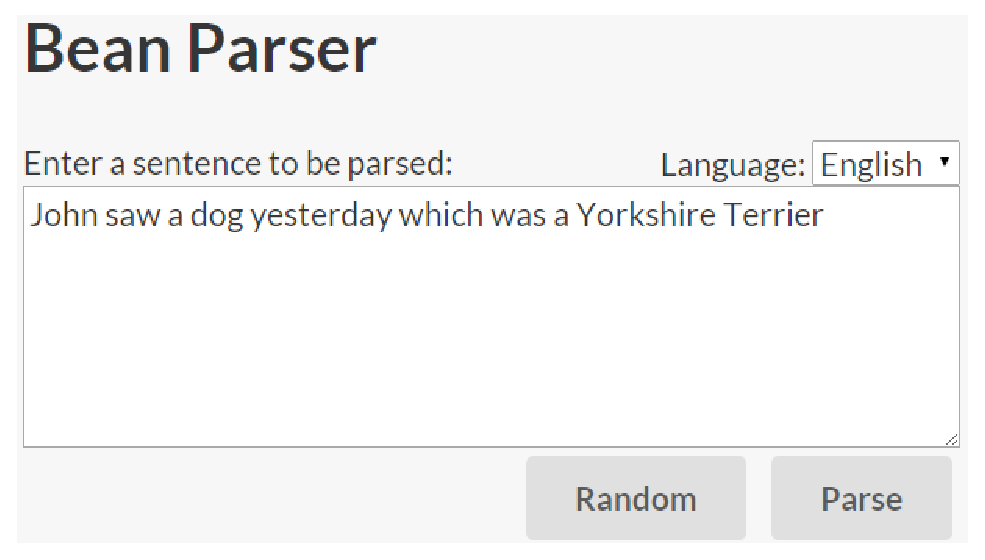
\epsfig{file=inputshot.eps, width=0.8\columnwidth}
	\caption{Snapshot of our demo website}
	\label{fig:demo1}
\end{figure}


\begin{figure}[th]
	\centering
	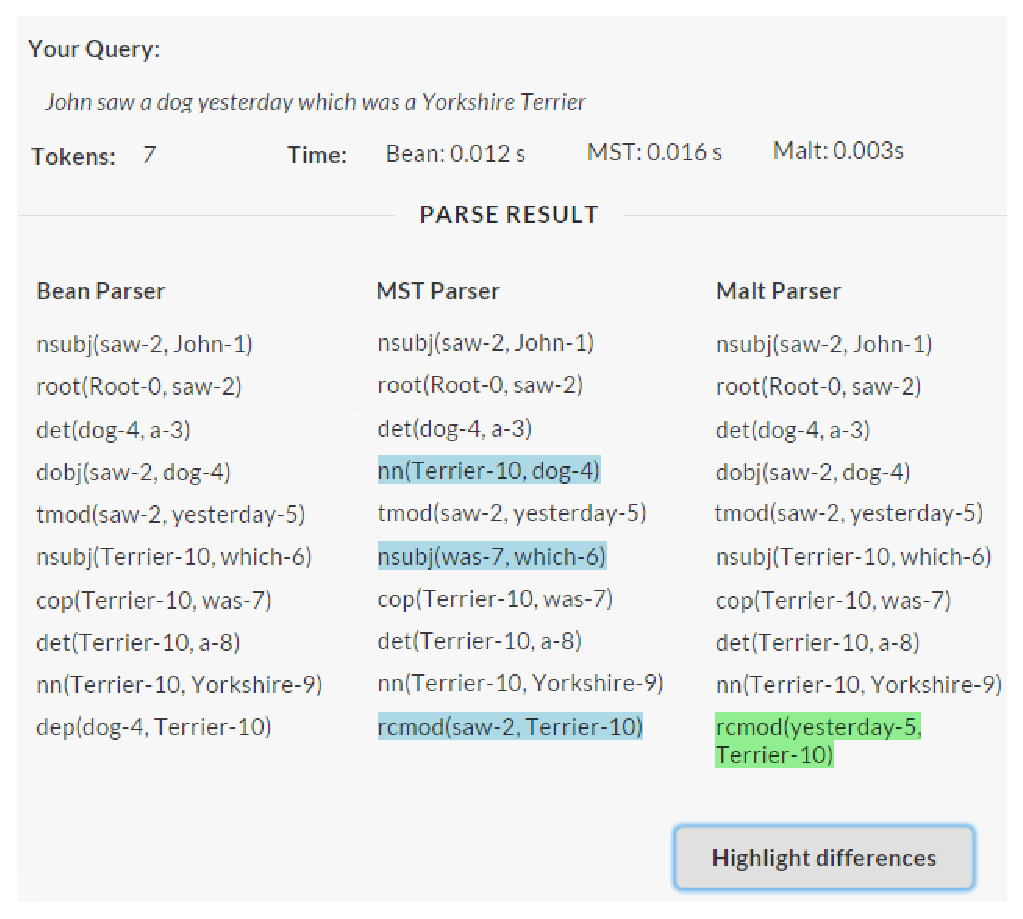
\epsfig{file=resultshot.eps, width=\columnwidth}
	\caption{Demo query result}
	\label{fig:demo2}
\end{figure}
}


% Table generated by Excel2LaTeX from sheet 'Sheet2'



%\BF{accuracy table: wsj, conll2007. current best, advantage in non-proj, progress in two
%components will enhance overall accuracy,view the}
